\documentclass[a4paper, 11pt]{article}
\usepackage{comment} 
\usepackage{lipsum} %This package just generates Lorem Ipsum filler text. 
\usepackage{fullpage} % changes the margin
\usepackage[a4paper, total={7in, 10in}]{geometry}
\usepackage[fleqn]{amsmath}
\usepackage{amssymb,amsthm}  % assumes amsmath package installed
\newtheorem{theorem}{Theorem}
\newtheorem{corollary}{Corollary}
\usepackage{graphicx}
\usepackage{tikz}
\usetikzlibrary{arrows}
\usepackage{verbatim}
\usepackage[numbered]{mcode}
\usepackage{float}
\usepackage{tikz}
    \usetikzlibrary{shapes,arrows}
    \usetikzlibrary{arrows,calc,positioning}

    \tikzset{
        block/.style = {draw, rectangle,
            minimum height=1cm,
            minimum width=1.5cm},
        input/.style = {coordinate,node distance=1cm},
        output/.style = {coordinate,node distance=4cm},
        arrow/.style={draw, -latex,node distance=2cm},
        pinstyle/.style = {pin edge={latex-, black,node distance=2cm}},
        sum/.style = {draw, circle, node distance=1cm},
    }
\usepackage{xcolor}
\usepackage{mdframed}
\usepackage[shortlabels]{enumitem}
\usepackage{indentfirst}
\usepackage{hyperref}
\usepackage[capitalize, nameinlink]{cleveref}
\renewcommand{\thesubsection}{\thesection.\alph{subsection}}

\newenvironment{problem}[2][Problem]
    { \begin{mdframed}[backgroundcolor=gray!20] \textbf{#1 #2} \\}
    {  \end{mdframed}}

\newenvironment{reduction}
    { \begin{mdframed}[backgroundcolor=blue!20] \\}
    {  \end{mdframed}}
% Define solution environment

\newcommand{\hr}{\noindent\rule{7in}{2.8pt}}
\newenvironment{solution}
    {\textit{Solution:}}
    {\clearpage}
\newcommand{\prob}[1]{\begin{mdframed}[backgroundcolor=gray!20] \textbf{Problem #1}\end{mdframed}}
\renewcommand{\qed}{\quad\qedsymbol}
\newcommand{\bit}{\left\{0, 1\right\}}
\newcommand{\enc}{\mathsf{Enc}}
\newcommand{\dec}{\mathsf{Dec}}
\newcommand{\negl}{\mathsf{negl}}
\newcommand{\prf}{\mathsf{PRFAdv}}
\newcommand{\prg}{\mathsf{PRGAdv}}
\newcommand{\poly}{\mathsf{poly}}
\newcommand{\N}{\mathbb{N}}
\newcommand{\R}{\mathbb{R}}
\newcommand{\Z}{\mathbb{Z}}

\newcommand{\calA}{\mathcal{A}}
\newcommand{\calB}{\mathcal{B}}
\newcommand{\calC}{\mathcal{C}}
\newcommand{\calE}{\mathcal{E}}
\newcommand{\calF}{\mathcal{F}}
\newcommand{\calG}{\mathcal{G}}
\newcommand{\calH}{\mathcal{H}}
\newcommand{\calK}{\mathcal{K}}
\newcommand{\calM}{\mathcal{M}}
\newcommand{\calS}{\mathcal{S}}
\newcommand{\calX}{\mathcal{X}}
\newcommand{\calY}{\mathcal{Y}}

\newcommand{\inparen}[1]{\left{ #1 \right}}
\newcommand{\probtwo}[2]{\mathsf{Pr}_{#1}\left[ #2 \right]}
\newcommand{\set}[1]{\left\{ #1 \right\}}
\newcommand{\ct}{\mathsf{ct}}
\newcommand{\twotimessadv}[1]{\mathsf{2SSAdv}\left[ #1 \right]}



\newlength{\protowidth}
\newcommand{\pprotocol}[5]{
{\begin{figure*}[#3]
\begin{center}
\setlength{\protowidth}{\textwidth}
\addtolength{\protowidth}{-3\intextsep}

\fbox{
        \small
        \hbox{\quad
        \begin{minipage}{\protowidth}
    \begin{center}
    {\bf #1}
    \end{center}
        #5
        \end{minipage}
        \quad}

        }
        
\end{center}
\vspace{-4ex}
\caption{{#4} #2}
\end{figure*}
} }

% the first arg is name of security game
% the second arg is caption
% the third arg is the game description
% the label needs to be included 
\newcommand{\securitygame}[4]{
   \pprotocol{#1}{#2}{ht!}{#3}{#4}
}

\newcommand{\constr}[4]{
   \pprotocol{#1}{#2}{tbh!}{#3}{#4}
}

\begin{document}

\noindent
\large\textbf{Anish Banerjee, Shankh Gupta} \hfill \textbf{Problem Set - 1}   \\
\normalsize COL759: Cryptography \hfill August 2023\\
\hr


\prob{1: Perfect 2 time security}
\begin{solution}

\end{solution}


\prob{2 : Secure/Insecure PRGs and PRFs}
\begin{solution}
    \begin{enumerate}[(a)]
        \item PRGs
              \begin{enumerate}[i.]
                  \item $\calG' = \set{G'_n : \bit^{2n} \to \bit^{3n}}_{n \in \N}$, where $$ G'_n(s_1 ~||~ s_2) = G_n(s_1) \wedge G_n(s_2).$$
                        The given PRG is \textbf{insecure}. Consider the PRG game between $\calA$ and $G'$ challenger where on input $y$, $\calA$ outputs the last bit of $y$. Let $L(x)$ denote the last bit of $x$. Note that if $G$ is secure, then $\Pr[L(G(s)=0)]$ will be close to 1/2. Otherwise, if it is $1/2+\epsilon$ we can create an adversary breaking $G$ with non-negligible advantage $\epsilon$($\calA$ always outputs 0). So, if we take $\Pr[L(G(s))=0]=1/2+\negl(\lambda)$
                        $$\Pr[b'=0|b=0]=\Pr[L(G(s_1)\wedge G(s_2))=0]$$
                        $$\leq\Pr[L(G(s_1))=0\wedge L(G(s_2))=0]+\Pr[L(G(s_1))=1\wedge L(G(s_2))=0]+\Pr[L(G(s_1))=0\wedge L(G(s_2))=1]$$
                        $$\approx3/4+\negl(\lambda)$$
                        and
                        $$\Pr[b'=0|b=1]=1/2$$
                        Thus the $\prg[\calA,\calG]\approx1/4$ which is non-negligible.

                  \item $\calG' = \set{G'_n : \bit^{2n} \to \bit^{3n}}_{n \in \N}$, where $$ G'_n(s_1 ~||~ s_2) = G_n(s_1) \oplus G_n(s_2)$$
                        This is a \textbf{secure} PRG. We prove the security by a hybrid argument.
                        \begin{itemize}
                            \item\textbf{World0} The challenger sends $G_n(s_1) \oplus G_n(s_2)$ to the attacker

                            \item\textbf{HybridWorld} The challenger sends $G_n(s_1) \oplus \mathsf{random}_1$ to the attacker

                            \item\textbf{World1} The challenger sends $\mathsf{random}_1\oplus\mathsf{random}_2$ to the attacker

                        \end{itemize}
                        \paragraph{Claim:} If any adversary $\calA$ can distinguish between World0 and HybridWorld then we can construct $\calB$ which breaks the PRG security of $G$. 

                        The reduction $\calB$ receives $y$ from the PRG challenger. It samples $s\gets\bit^n$ and sends $G(s)\oplus y$ to $\calA$. The advantage of $\calA$ in distinguishing between World0 and HybridWorld will be equal to the advantage of $\calB$ in breaking PRG security of $G$. 
                        
                        Similarly we can also claim that:

                        \paragraph{Claim:} If any adversary $\calA$ can distinguish between HybridWorld and World1 then we can construct $\calB$ which breaks the PRG security of $G$.

                        The reduction $\calB$ receives $y$ from the PRG challenger. It samples $r\gets\bit^n$ and sends $r\oplus y$ to $\calA$. The advantage of $\calA$ in distinguishing between HybridWorld and World1 will be equal to the advantage of $\calB$ in breaking PRG security of $G$.

                        Now we can choose any reduction randomly to break the PRG security of $G$. Also note that we cannot use a similar argument in part i. because $\mathsf{random}_1\wedge\mathsf{random}_2$ is not truely random

              \end{enumerate}
        \item PRFs
              \begin{enumerate}[i.]
                  \item $\calF' = \set{F'_n:\bit^{n} \times \bit^{2n} \to \bit^{n}}_{n\in \N}$ where $$F'_n(k, (x_1, x_2)) = F_n(k, x_1) \oplus F_n(k, x_2).$$

                        The given family $\calF'$ is \textbf{insecure}. Consider a PPT attacker $\calA$ who sends $\poly(\lambda)$ distinct $(x_i,x_i)$ queries to the  challenger. If the challenger chooses $b=0$ then it will end up sending $$F_n(k, x_i) \oplus F_n(k, x_i)=0^n$$ for each of the queries. The attacker outputs 0 if all the responses are 0 and 1 otherwise. Advantage of the attacker is close to 1, precisely $1-2^{-n\poly(\lambda)}$.

                  \item $\calF' = \set{F'_n:\bit^{n} \times \bit^{n} \to \bit^{n}}_{n\in \N}$ where $$F'_n(k, x) = F_n(k, x) \oplus x.$$

                        The given family is \textbf{secure}. Given an adversary $\calA$ which breaks PRF security of $\calF'$, we can construct an adversary $\calB$ which breaks the security of $\calF$ (\cref{red:p2bii})
                        \securitygame{Problem 2(b)(ii)}{Reduction for Problem 2(b)(ii)}{\label{red:p2bii}}
                        {
                            \begin{itemize}
                                \item Challenger picks a uniformly random bit $b \gets \bit$ and a seed $s\gets \bit^n$.
                                \item The adversary $\calA$ makes polynomially many queries to $\calB$, who passes them to the challenger. Challenger replies as in the PRF Game.
                                \item Upon receiving the response $y_i$ of each query, $\calB$ sends $ y_i\oplus x_i$ to $\calA$
                                \item After polynomially many queries, $\calB$ forwards the response send by $\calA$ $(b')$ and wins if $b=b'$.
                            \end{itemize}
                        }

              \end{enumerate}
    \end{enumerate}

\end{solution}

\prob{3 : PRG Security does not imply Related-Key-PRG Security}
\begin{solution}

\end{solution}


\prob{4 : Constructing PRFs from PRGs}
\begin{solution}
    We will use a tree construction similar to the one given in the book (\cref{fig:TC})
    \begin{figure}[!ht]
        \centering
        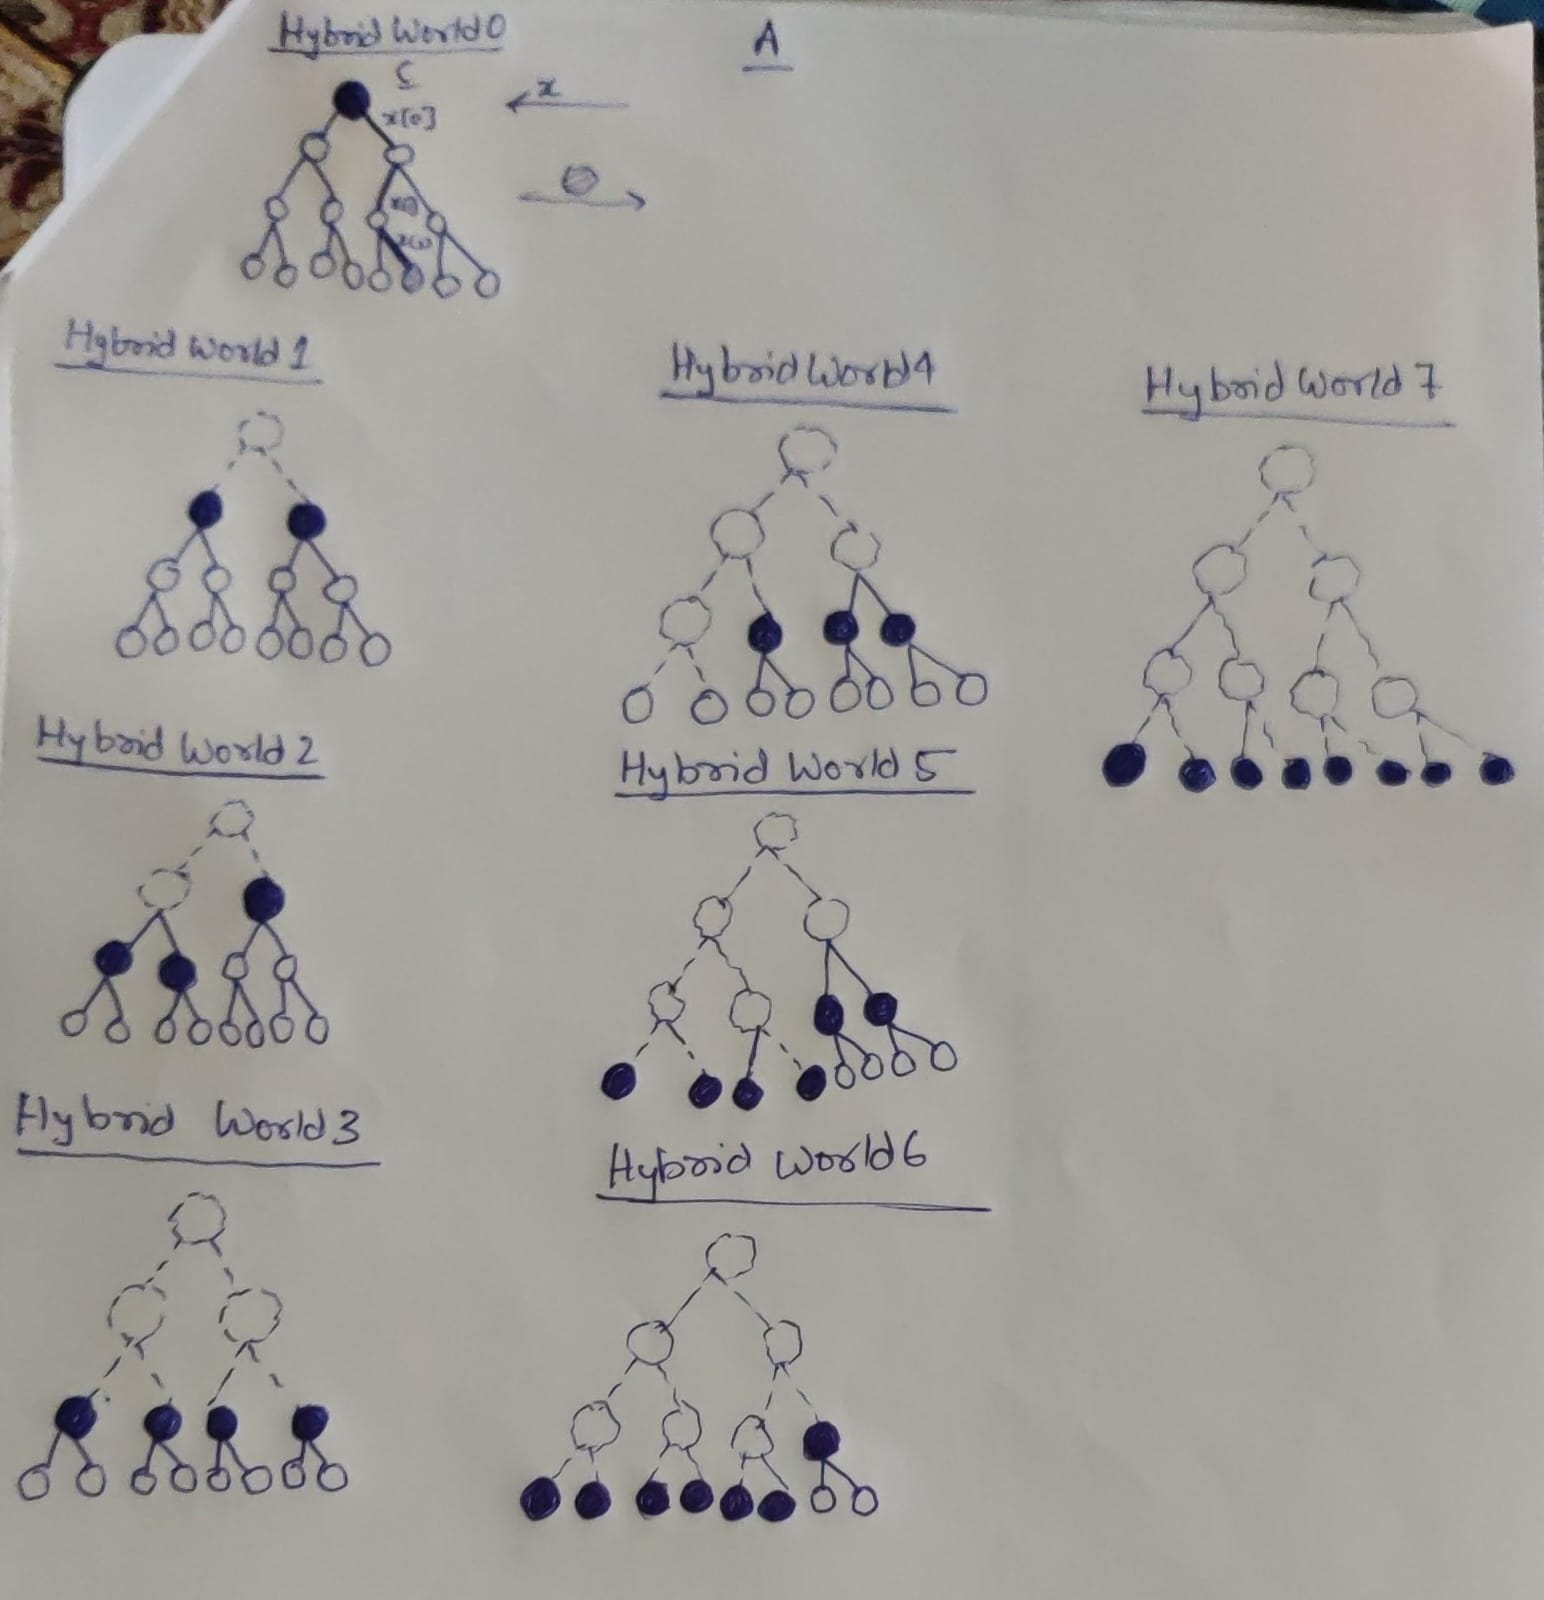
\includegraphics[scale=0.25]{images/Tree Construction.png}
        \caption{Construction of Hybrid worlds for the case $\log n=3$. The randomly generated nodes are shadedand the nodes which can be ignored are dotted}
        \label{fig:TC}
    \end{figure}
    \begin{enumerate}[(a)]
        \item  Construct $n$ hybrid worlds in the following way: In Hybrid $j$, the challenger builds an evaluation tree whose nodes are labeled as follows:
              \begin{itemize}
                  \item The first $j$ nodes (as appearing in the level order traversal of the tree) can be ignored.
                  \item The next $j + 1$ nodes are labelled with random values. 
                  \item Remaining nodes are derived from their parents.
              \end{itemize}
              In response to a query $x\in\bit^{\log n}$ in Hybrid $j$, the challenger sends to the adversary the label of the leaf addressed by $x$.

              Observe that Hybrid $0$ corresponds to the case $b=0$ in the PRF game when the challenger sends $F_k(x)$ and Hybrid $l$ corresponds to $b=1$ when the challenger uses a truly random function.

              \paragraph{Claim:} If there exists an adversary $\calA$ which can distinguish between Hybrid $i$ and Hybrid $i+1$ then we can construct an adversary $\calB$ which breaks the PRG security of $G$.

              \textit{Proof:} Consider the reduction \cref{red:p4a}

              \securitygame{Problem 4(a)}{Reduction for Problem 4(a)}{\label{red:p4a}}
              {
                  \begin{itemize}
                      \item Challenger picks a uniformly random bit $b \gets \bit$ and a seed $s\gets \bit^n$. If $b=0$, he sends $y=G(s)$ to $\calB$ otherwise he sends a $y=r\gets\bit^{2n}$.
                      \item $\calB$ constructs the evaluation tree. 
                      \begin{itemize}
                        \item The first $i+1$ nodes can be ignored
                        \item The next $i$ nodes are randomly generated
                        \item The next two nodes are made by splitting $y$ sent by the challenger into two halves
                        \item Remaining nodes are generated using the algorithm from their parents.
                      \end{itemize} 
                      \item The adversary $\calA$ makes polynomially many queries to $\calB$. In response to a query $x\in\bit^{\log n}$, $\calB$ sends the label of the leaf addressed by $x$ (This traveral is shown in the HybridWorld0 of \cref{red:p4a})
                      \item After polynomially many queries, $\calB$ forwards the response send by $\calA$ $(b')$ and wins if $b=b'$.
                  \end{itemize}
              }
              \begin{figure}[!ht]
                \centering
                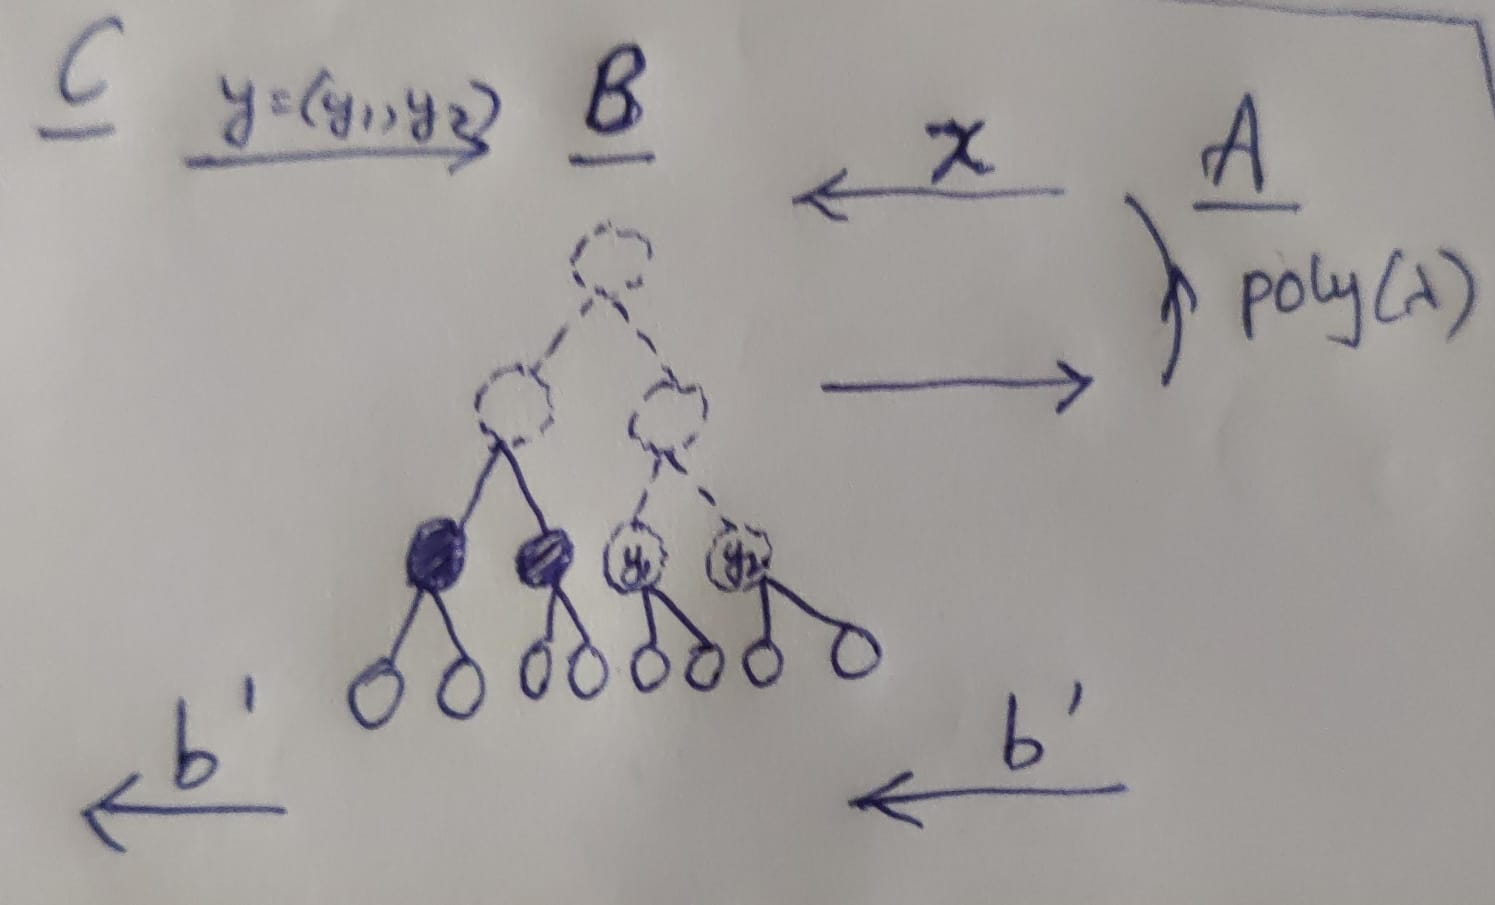
\includegraphics[scale=0.25]{images/Tree Red.png.jpg}
                \caption{Reduction for distinguishing between HybridWorld2 and HybridWorld3}
                \label{fig:p4a2}
              \end{figure}


                  From the construction, it can be checked that:
                  $$\Pr[b'=0|b=0]=\Pr[\calA\text{ outputs 0 in HybridWorld } i]=p_{i}$$
                  $$\Pr[b'=0|b=0]=\Pr[\calA\text{ outputs 0 in HybridWorld } i+1]=p_{i+1}$$
                  Thus,
                  $$\prg[\calB,\calG]=|p_{i}-p_{i+1}|$$
                  Finally for the combined reduction, we choose any one of the reductions at random.
                  $$\prg[\calB^c,\calG^c]=\frac{|p_{l}-p_{0}|}{\log n}$$
        \item In the above construction, $\calB$ will need to sample $O(2^d)$ random bitstrings in some hybrids, where $d$ is the depth of the tree. If $d=\log n$ then $\calB$ samples $O(n)$ bitstrings. However, if $d=n$ then he has to sample exponentially many strings, making him inefficient. So, we cannot use the same reduction when $x\in\bit^n$.
        \item The given construction is insecure. Consider an adversary $\calA$ which plays the following game $\calG$:
              \begin{itemize}
                  \item $\calA$ sends $x$ to the Challenger and receives $y_1$
                  \item $\calA$ sends $x||1$ to the Challenger and receives $y_2$
                  \item $\calA$ finds $G(y_1)=(s_0,s_1)$ and checks if $s_1=y_1$. If so it returns $b'=0$ else $b'=1$
              \end{itemize}
              Now,
              $$\prf[\calA,\calG]=|\Pr[b'=0|b=0]-\Pr[b'=0|b=1]|$$
              From construction we have,
              $$\Pr[b'=0|b=0]=1$$
              and
              $$\Pr[b'=0|b=1]=\Pr[G(y_1)=(s_0,s_1)\wedge s_1=y_1]=2^{-n}$$
              Thus the $\prf[\calA,\calG]=1-2^{-n}$
    \end{enumerate}
\end{solution}


\end{document}
